\documentclass[main.tex]{subfiles}
\begin{document}
\section{Transférer}
%%%%%%%%%%%%%%%%%%%%%%%%%%%%%%%%%%%%%%%
% EXERCICE
\begin{exercise}[points=5]
    Voici, pour la production de l'année 2021, le relevé
    des longueurs des gousses de vanille d'un cultivateur
    de Tahaa.
    \begin{center}
        \begin{tblr}{hlines, vlines, columns={r, 1cm}, column{1}={l, 2.5cm}}
            Longueur (cm) & 12        & 15        & 17          & 22          & 23        \\
            Effectif      & \num{600} & \num{800} & \num{1 800} & \num{1 200} & \num{600}
        \end{tblr}
    \end{center}

    \begin{enumerate}
        \item Quel est l'effectif total de cette production ?
        \item Détermine l'étendue de cette série.
        \item Le cultivateur peut seulement conditionner les
              gousses de vanille dans des tubes de \SI{20}{cm} de
              long. Quel pourcentage de cette production a-t-il
              pu conditionner sans plier les gousses ?
        \item La chambre d'agriculture décerne une récompense
              (un \og label de qualité \fg{}) aux agriculteurs si :
              \begin{itemize}
                  \item  la longueur moyenne des gousses de leur
                        production est supérieure ou égale à \SI{16,5}{cm} ;
                  \item plus de la moitié des gousses de leur
                        production a une taille supérieure à \SI{17,5}{cm}.
              \end{itemize}
              Ce cultivateur pourra-t-il recevoir ce \og label de
              qualité \fg{} ?
    \end{enumerate}
\end{exercise}
% SOLUTION
\begin{solution}

\end{solution}
%%%%%%%%%%%%%%%%%%%%%%%%%%%%%%%%%%%%%%%
% EXERCICE
\newpage
\begin{exercise}[points=4]
    L'entraîneur de l'équipe de football de Sésaville compare le nombre de tirs effectués par ses
    trois attaquants pendant la première moitié du championnat.
    \begin{center}
        \pgfplotsset{width=.5\linewidth}
        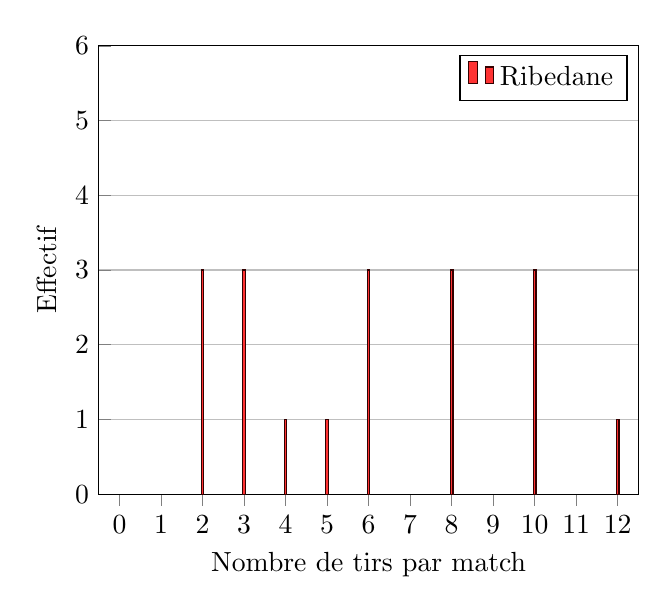
\begin{tikzpicture}
    \begin{axis}[
            ybar,
            xmin=-0.5,
            ymin=0,
            xmax=12.5,
            ymax=6,
            xlabel=Nombre de tirs par match,
            ylabel=Effectif,
            bar width=1pt,
            %major grid style={draw=black},
            ymajorgrids = true,
            xtick pos=bottom,
            ytick pos=left,
            %minor y tick num = 4,
            %minor y tick style = {transparent},
            %major x tick style = {transparent},
            %yminorticks = true,
            %yminorgrids = true,
            xtick distance=1,
            ytick distance=1,
            %axis lines* = left
        ]
        \addplot[red!20!black,fill=red!80!white] coordinates{
                (2,3)
                (3,3)
                (4,1)
                (5,1)
                (6,3)
                (8,3)
                (10,3)
                (12,1)
            };
        \legend{Ribedane}
    \end{axis}
\end{tikzpicture}
        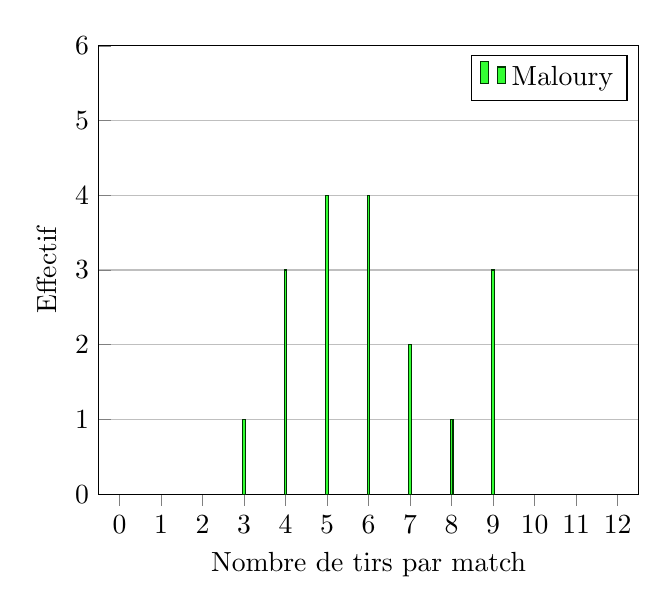
\begin{tikzpicture}
    \begin{axis}[
        ybar,
        xmin=-0.5,
        ymin=0,
        xmax=12.5,
        ymax=6,
        xlabel=Nombre de tirs par match,
        ylabel=Effectif,
        bar width=1pt,
        %major grid style={draw=black},
        ymajorgrids = true,
        xtick pos=bottom,
        ytick pos=left,
        %minor y tick num = 4,
        %minor y tick style = {transparent},
        %major x tick style = {transparent},
        %yminorticks = true,
        %yminorgrids = true,
        xtick distance=1,
        ytick distance=1,
        %axis lines* = left
    ]
        \addplot[green!20!black,fill=green!80!white] coordinates{
               (3,1)
               (4,3)
               (5,4)
               (6,4)
               (7,2)
               (8,1)
               (9,3)
            };
            \legend{Maloury}
    \end{axis}
\end{tikzpicture}
        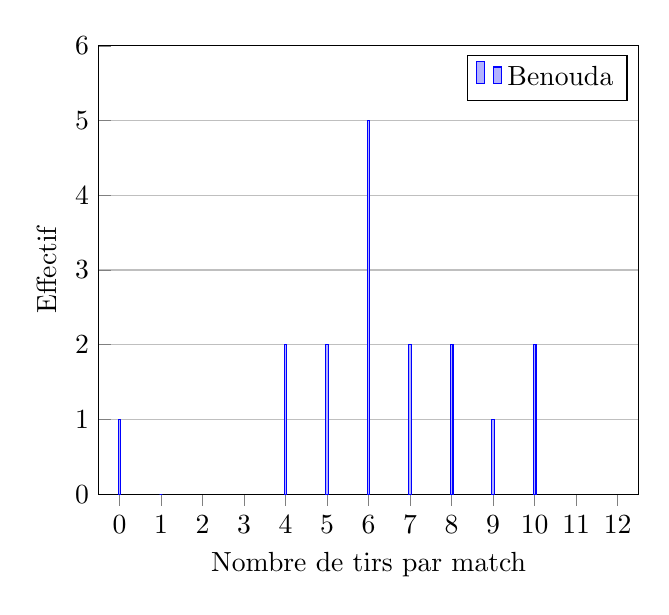
\begin{tikzpicture}
    \begin{axis}[
        ybar,
        xmin=-0.5,
        ymin=0,
        xmax=12.5,
        ymax=6,
        xlabel=Nombre de tirs par match,
        ylabel=Effectif,
        bar width=1pt,
        %major grid style={draw=black},
        ymajorgrids = true,
        xtick pos=bottom,
        ytick pos=left,
        %minor y tick num = 4,
        %minor y tick style = {transparent},
        %major x tick style = {transparent},
        %yminorticks = true,
        %yminorgrids = true,
        xtick distance=1,
        ytick distance=1,
        %axis lines* = left
    ]
        \addplot coordinates{
                (0,1)
                (1,0)
                (4,2)
                (5,2)
                (6,5)
                (7,2)
                (8,2)
                (9,1)
                (10,2)
            };
            \legend{Benouda}
    \end{axis}
\end{tikzpicture}
    \end{center}
    %\pgfplotsset{width=.5\linewidth}

    \begin{enumerate}
        \item Calcule le nombre de tirs au but moyen par match des trois attaquants.
        \item  Détermine le nombre de tirs au but médian pour chacune de ces trois séries.
        \item Quel buteur prendrais-tu dans ton équipe ? Justifie en utilisant les résultats obtenus aux sous-questions précédentes.
    \end{enumerate}
\end{exercise}
% SOLUTION
\begin{solution}

\end{solution}
\end{document}